% $Header$

\documentclass{beamer}

% Copyright (c)  2021  HiKlas Ltd.
% Permission is granted to copy, distribute and/or modify this document
% under the terms of the GNU Free Documentation License, Version 1.3
% or any later version published by the Free Software Foundation;
% with no Invariant Sections, no Front-Cover Texts, and no Back-Cover Texts.
% A copy of the license is included in the section entitled "GNU
% Free Documentation License".
%
% Based on the Beamer generic-ornate-15min-45min.en.tex template by
% Till Tantau <tantau@users.sourceforge.net>



\mode<presentation>
{
  \usetheme{CambridgeUS}
}

\usepackage[english]{babel}
\usepackage[latin1]{inputenc}
\usepackage[T1]{fontenc}
% Or whatever. Note that the encoding and the font should match. If T1
% does not look nice, try deleting the line with the fontenc.

% These packages are used for drawing circuits
\usepackage{tikz}
\usepackage[siunitx,european,americanresistors]{circuitikz}
\usetikzlibrary{circuits.logic.US}

% Packages for mathematical notation
\usepackage{amsmath}

% Packages for including graphics images
\usepackage{graphics}

% Packages for misc purposes
\usepackage{siunitx}


% Information about the presentation 
\title{Introduction to Machine Code}
\subtitle{001 Overview}
\author{Fiona Bianchi}
\institute{HiKlas Ltd}
\date{August 2021}
\subject{Talks}
\pgfdeclareimage[height=0.5cm]{company-logo}{../assets/HiklasLogo.eps}
\logo{\pgfuseimage{company-logo}}

% Table of contents for each Subsection
\AtBeginSubsection[]
{
  \begin{frame}<beamer>{Outline}
    \tableofcontents[currentsection,currentsubsection]
  \end{frame}
}

% TODO: Nope, I don't think I want this put leaving it in just in case
% TODO: to remove when absolutely sure
% If you wish to uncover everything in a step-wise fashion, uncomment
% the following command: 
%\beamerdefaultoverlayspecification{<+->}


\begin{document}

\begin{frame}
  \titlepage
\end{frame}

\begin{frame}{Outline}
  \tableofcontents
  % TODO: What is "pausesections" for?
  % You might wish to add the option [pausesections]
\end{frame}


\section{Back to Basics}

\subsection[Switches]{Simple Electronics Switches}

\begin{frame}{A Light Switch}

  \begin{columns}
    \column{0.5\textwidth}
    \begin{itemize}
    \item
      The simplest electronic cicruit
    \item
      Switch has two positions, ``on'' or ``off''
    \item
      What has this got to do with computers?
    \end{itemize}

    \column{0.5\textwidth}
    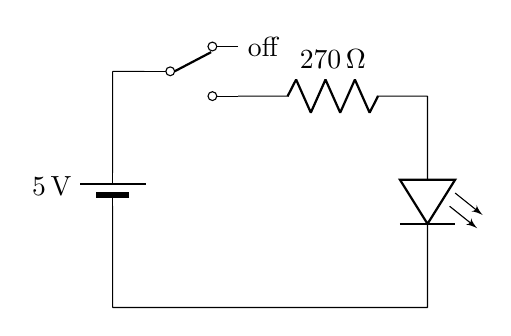
\begin{tikzpicture}
      \coordinate (as) at (4,3);
      \draw 
	(0, 3) to [battery2, l_=5<\volt>,] (0,0) 
	(1, 3) node[spdt] (Sw1) {}
	(0, 3) to [short] (Sw1.in)
		(Sw1.out 1) node[right] {off} 
	(Sw1.out 2) to [R,label=270<\ohm>] (as |- Sw1.out 2)
	(as |- Sw1.out 2) to [empty led] (4,0)
	(4,0) to (0,0);
    \end{tikzpicture}
  \end{columns}
\end{frame}


\begin{frame}{A Backwards Light Switch}

  \begin{columns}
    \column{0.5\textwidth}
    \begin{itemize}
    \item
      Someone wires a switch wrongly
    \item
      You have to flick it to ``off'' to switch the light on 
    \item
      This is backwards, or the inverse of what we'd expect
    \end{itemize}

    \column{0.5\textwidth}
    \resizebox{\textwidth}{!}{
      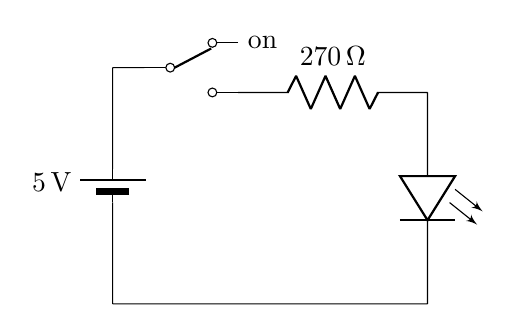
\begin{tikzpicture}
        \coordinate (as) at (4,3);
        \draw 
	(0, 3) to [battery2, l_=5<\volt>,] (0,0) 
	(1, 3) node[spdt] (Sw1) {}
	(0, 3) to [short] (Sw1.in)
		(Sw1.out 1) node[right] {on} 
	(Sw1.out 2) to [R,label=270<\ohm>] (as |- Sw1.out 2)
	(as |- Sw1.out 2) to [empty led] (4,0)
	(4,0) to (0,0);
      \end{tikzpicture}
      }
  \end{columns}
\end{frame}


\begin{frame}{Both Light Switches On}

  \begin{columns}
    \column{0.5\textwidth}
    \begin{itemize}
    \item
      Two switches in series (one after the other)
    \item
      You have to flick both to ``on'' for the lamp to work 
    \item
      Switch 1 AND Switch 2
    \end{itemize}

    \column{0.5\textwidth}
    \resizebox{\textwidth}{!}{
      \begin{tikzpicture}
        \coordinate (as) at (6,4);
        \draw 
	(0, 4) to [battery2, l_=5<\volt>,] (0,0) 
	(1, 4) node[spdt] (Sw1) {}
	(3,4) node[spdt, xscale=-1] (Sw2) {}
	(0, 4) to [short] (Sw1.in)
		(Sw1.out 1) node[right] {off}
	(Sw1.out 2) to (Sw2.out 2) 
	(Sw2.in) to [R,label=270<\ohm>] (as)
	(as) to [empty led] (6,0)
	(6,0) to (0,0);
      \end{tikzpicture}
      }
  \end{columns}
\end{frame}


\begin{frame}{More Switches, but Why?}
  \begin{itemize}
  \item
    We can have switches in parallel so if either is ``on'' the LED lights, this is OR
  \item
    We can have one switch in series with two in parallel - OR and AND
  \item
    We could have lots and lots of switches making up quite complicated circuits
  \item
    Why would we do that though?  How does this related to computers or programming?
  \end{itemize}
\end{frame}


\subsection[Maths]{Doing Some Sums}

\begin{frame}{How To Add Two Numbers Together}
  \begin{columns}
    \column{0.75\textwidth}
    \begin{itemize}
    \item
      Start with the units (0-9) 
    \item
      Next move onto 10s (carry any extra 10s from units)
    \item
      Then hundreds (again adding in any 100s carried from 10s)
    \item
      And so on\dots
    \item
      Maths that most of us learn how to do and some still use\dots
    \item
      Well all of us still use, even if you didn't know you did
    \end{itemize}

    \column{0.25\textwidth}
    \begin{equation*}
      \begin{array}{c}
        \phantom{+9}3141\\
        \underline{+\phantom{99}271}\\
        \phantom{+9}3412\\
      \end{array}
    \end{equation*}
  \end{columns}
  
\end{frame}


\begin{frame}{How Many Fingers}
  \begin{itemize}
  \item
    We all use 10 as the basis for counting - 10 fingers, 10 toes
  \item
    This is actually called base 10 in mathematics
  \item
    There are other numbers bases that are commonly used
    \begin{itemize}
    \item
      Base 12 well it was commonly used by Eygptians 
    \item
      Base 16 also called hexadecimal
    \item
      Base 8 also called octal
    \item
      Base 2 also called binary
    \end{itemize}
  \item
    The last one is most interesting here
  \end{itemize}
\end{frame}


\begin{frame}{Binary Addition}
  \begin{columns}
    \column{0.75\textwidth}
    \begin{itemize}
    \item
      Start with the units (0-1) 
    \item
      Next move onto 2s (carry any extra 10s from units)
    \item
      Then 4s (again adding in any 4s carried from 2ss)
    \item
      And so on\dots
    \item
      Exactly the same rules with use for base 10
    \item
      The columns in binary aren't units, 10s, 100s, 1000s, etc
    \item
      Instead units (1s), 2s, 4s, 8s, 16s, 32s, 64s, 128s, 256s, etc
    \item
      64 binary digits can represent \num{1.84467e19}
    \end{itemize}

    \column{0.25\textwidth}
    \begin{equation*}
      \begin{array}{c}
        \phantom{+9}1101\\
        \underline{+\phantom{99}101}\\
        \phantom{+}10010\\
      \end{array}
    \end{equation*}
  \end{columns}
  
\end{frame}


\section{Logic}

\subsection[Putting It Together]{Binary Logic}

\begin{frame}{Switches And Binary}
  \begin{columns}
    \column{0.75\textwidth}
    \begin{itemize}
    \item
      Binary only has two digits, ``0'' and ``1'' 
    \item
      You can think of these as ``off'' and ``on'' for switches
    \item
      Electric circuits have a ``+'' and ``-'' (also known as ``+ve'' and ``\SI{0}{\volt}'')
    \item
      You can represents binary with ``+ve'' and ``\SI{0}{\volt}'', 1 and 0 respectively
    \item
      Binary logic can be implemented in electronics with switches
    \end{itemize}
    
    \column{0.25\textwidth}
    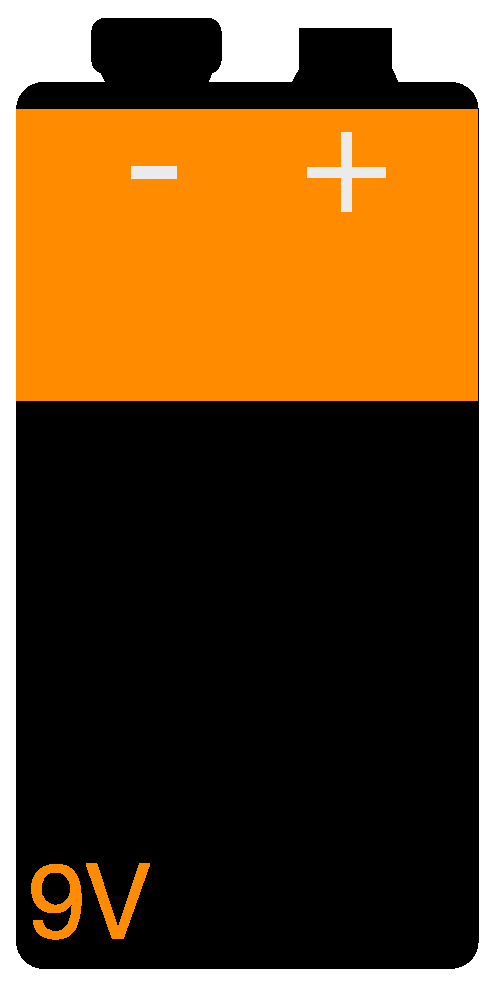
\includegraphics[scale=0.25]{../assets/9V-Battery.eps}
    
  \end{columns}
\end{frame}

\begin{frame}{Logic Levels}
  \begin{itemize}
  \item
    ``on'' is \SI{5}{\volt} or \SI{3.3}{\volt} or even \SI{1.8}{\volt}
  \item
    ``off'' is \SI{0}{\volt} (the negative terminal on a battery)
  \item
    ``on'' is 1 in binary 
  \item
    ``off'' is 0 in binary
  \item
    A single switch can be used to represent a binary digit (0 and 1)
  \item
    Two switches means 1s and 2s
  \item
    8 switches can represent any whole number between 0 and 255
  \end{itemize}
\end{frame}


\begin{frame}{Chips}
  \begin{columns}
    \column{0.7\textwidth}
    \begin{itemize}
    \item
      There were two main types TTL and CMOS
    \item
      Transistor Transistor Logic - now superceded
    \item
      Complimentary Metal Oxide Semiconductor
    \item
      Now almost everything is CMOS - don't touch!
    \item
      What is inside chips?
    \end{itemize}

    \column{0.3\textwidth}
    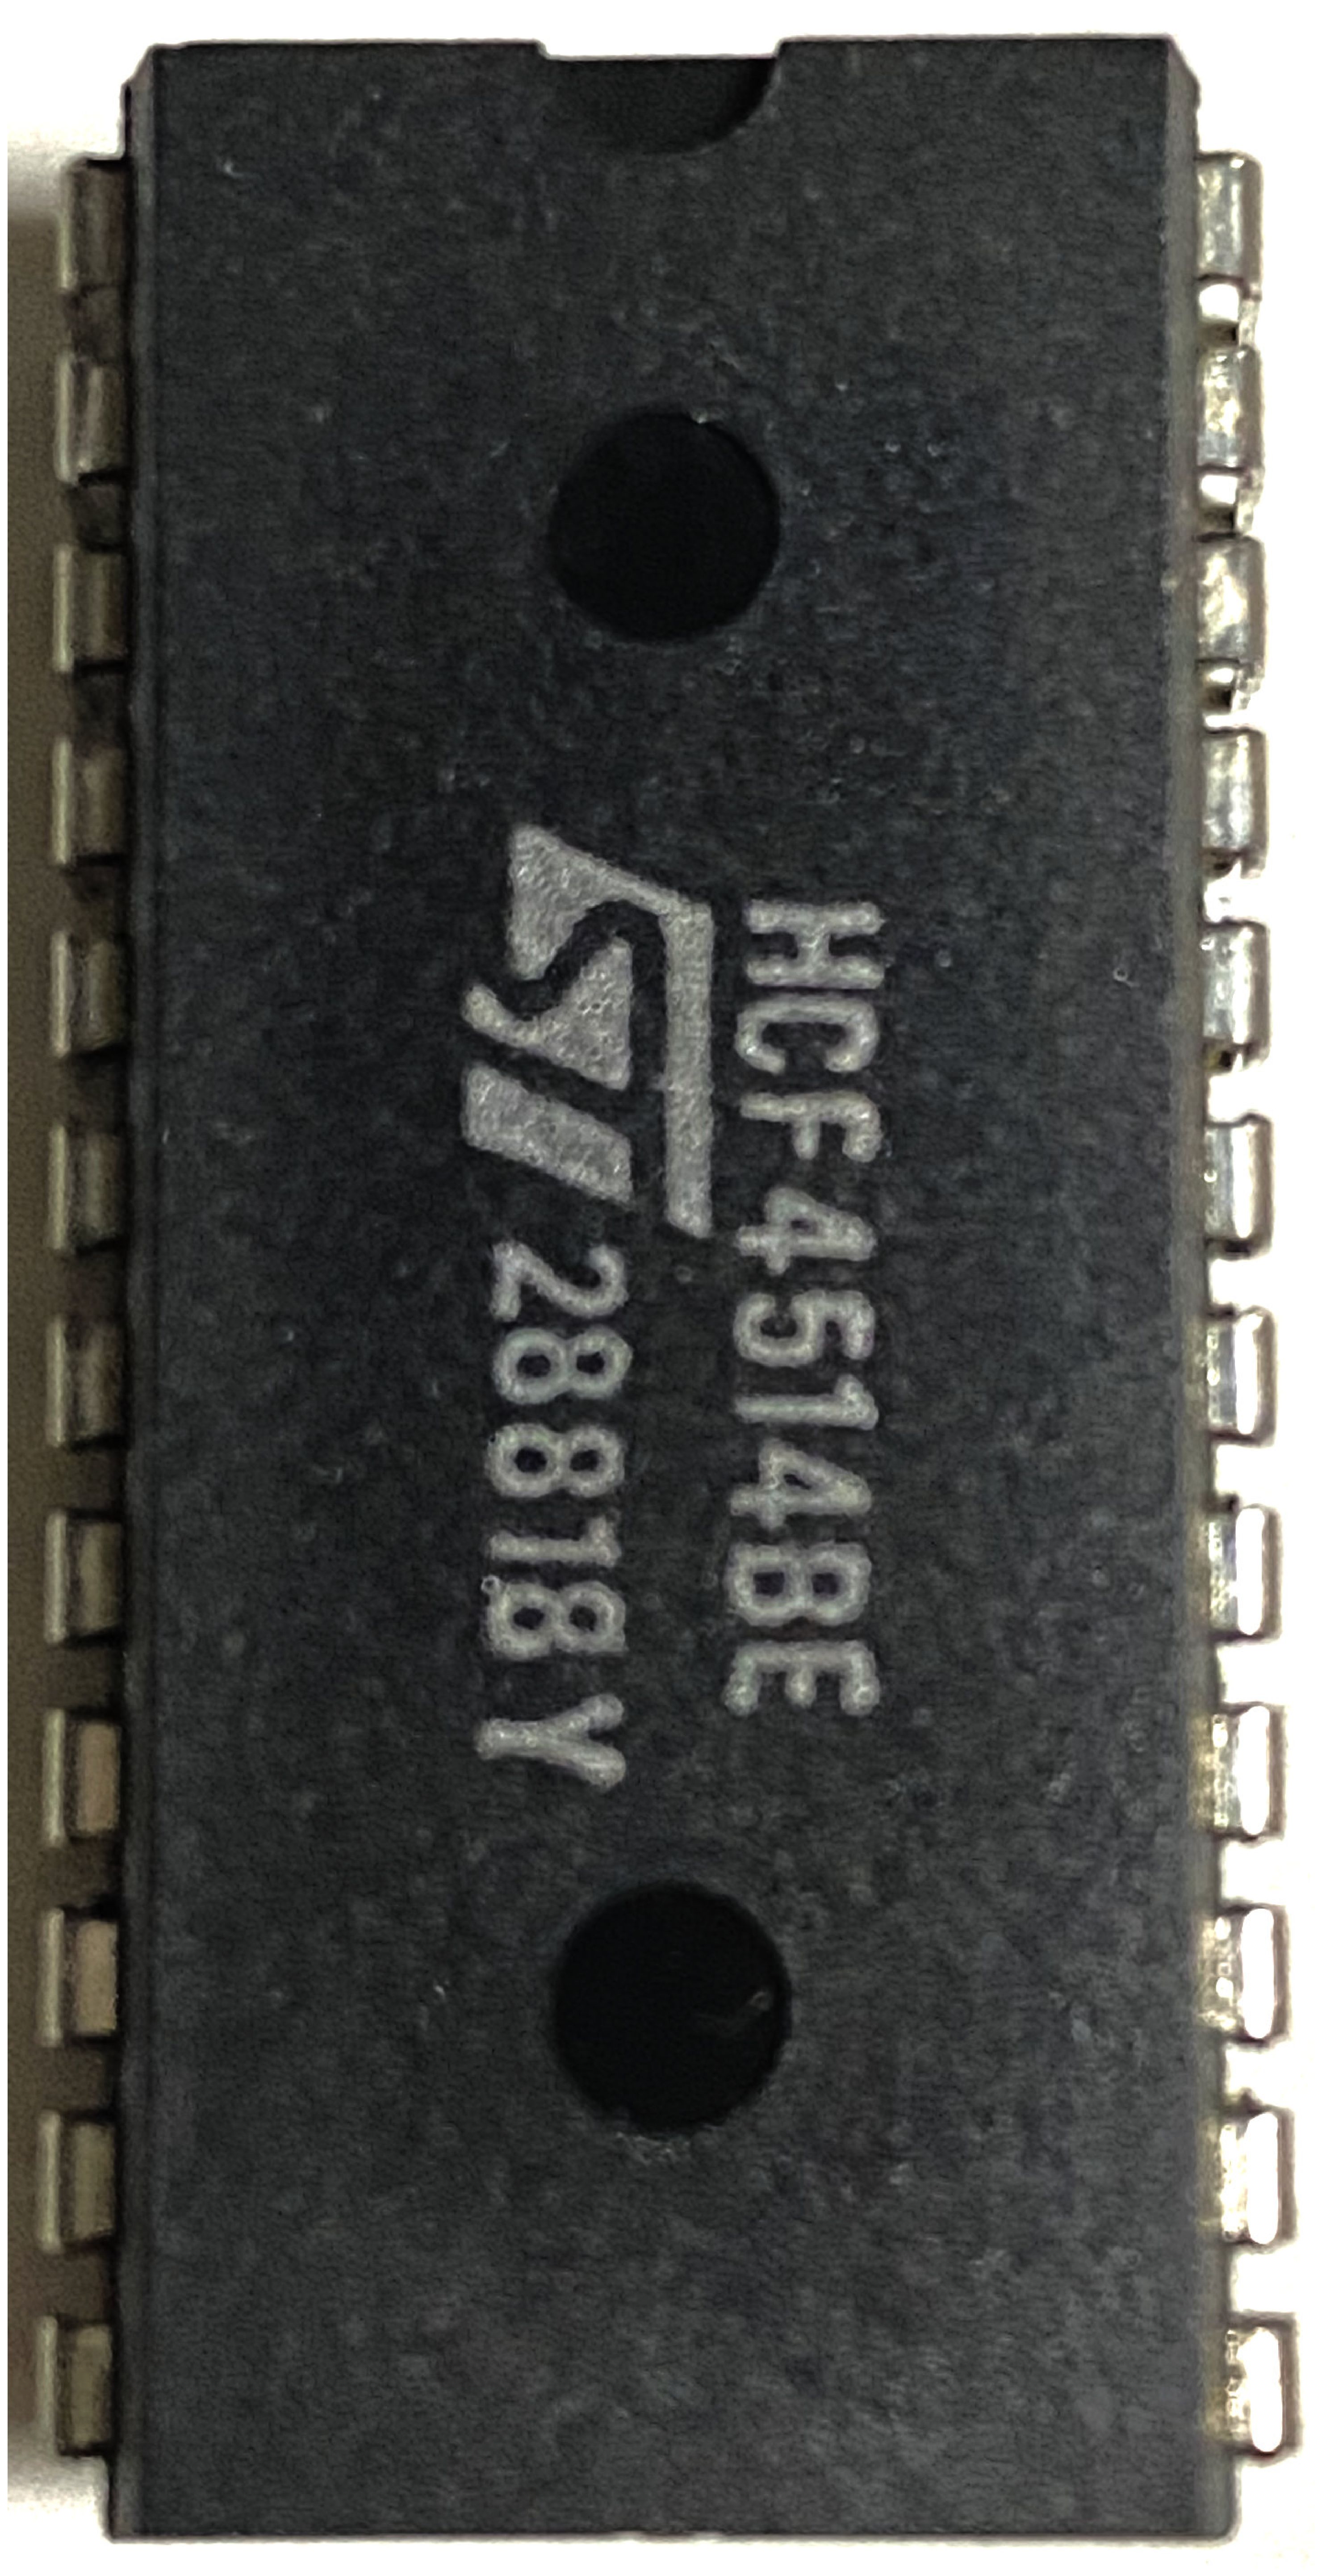
\includegraphics[scale=0.05]{../assets/IC-Picture.eps}
  \end{columns}    
\end{frame}


\begin{frame}{Logic Gates}
  \begin{itemize}
  \item
    Actually seen these before - switches
  \item
    Combinations of inputs result in outputs
  \item
    Two switches that both need to be ``on'' give logical AND
  \item
    Two switches either of which can be ``on'' is a logical OR
  \item
    Switches connect voltages (battery) to outputs which indicate logic levels/binary
  \item
    Chips can contain billions of switches, lets start small ...
  \end{itemize}
\end{frame}


\begin{frame}{AND Gate}
  \begin{columns}
    \column{0.7\textwidth}
    \begin{itemize}
    \item
      Both inputs must be ``on'' aka binary ``1''
    \item
      Output for this condition is ``1''
    \item
      For any other combination output is ``off'' aka binary ``0''
    \item
      Remember that ``1'' is also a certain voltage level and ``0'', is \SI{0}{\volt}
    \item
      Truth table shows the relationship between input and output
    \end{itemize}

    \column{0.3\textwidth}
    % TODO: Fix the input and output alignment, straighten the lines
    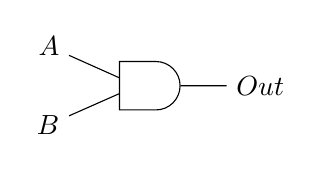
\begin{tikzpicture}[circuit logic US]
      \draw
      (1,1) node[and gate] (G) {}
      (0,1.5) node[anchor=east] (A) {$A$}
      (0,0.5) node[anchor=east] (B) {$B$}
      (2, 1) node[anchor=west] (O) {$Out$}
      (A) -- (G.input 1)
      (B) -- (G.input 2)
      (O) -- (G.output);
    \end{tikzpicture}
    % TODO: Add some spacing between diagram and table
    \begin{tabular}{ccc}
      \hline
      \textbf{A} & \textbf{B} & \textbf{Out} \\
      \hline
      0 & 0 & 0 \\
      0 & 1 & 0 \\
      1 & 0 & 0 \\
      1 & 1 & 1 \\
      \hline
    \end{tabular}    
  \end{columns}    
\end{frame}


\begin{frame}{OR Gate}
  \begin{columns}
    \column{0.7\textwidth}
    \begin{itemize}
    \item
      Either input can be ``on'' aka binary ``1''
    \item
      Output for this condition is ``1''
    \item
      You get a ``0'' or ``off'' only when both inputs are ``0''
    \item
      Again, the truth table shows the relationship between input and output
    \end{itemize}

    \column{0.3\textwidth}
    % TODO: Fix the input and output alignment, straighten the lines
    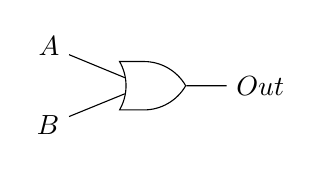
\begin{tikzpicture}[circuit logic US]
      \draw
      (1,1) node[or gate] (G) {}
      (0,1.5) node[anchor=east] (A) {$A$}
      (0,0.5) node[anchor=east] (B) {$B$}
      (2, 1) node[anchor=west] (O) {$Out$}
      (A) -- (G.input 1)
      (B) -- (G.input 2)
      (O) -- (G.output);
    \end{tikzpicture}
    % TODO: Add some spacing between diagram and table
    \begin{tabular}{ccc}
      \hline
      \textbf{A} & \textbf{B} & \textbf{Out} \\
      \hline
      0 & 0 & 0 \\
      0 & 1 & 1 \\
      1 & 0 & 1 \\
      1 & 1 & 1 \\
      \hline
    \end{tabular}    
  \end{columns}    
\end{frame}


\begin{frame}{More Logic Gates}
  \begin{itemize}
  \item
    ``AND'' and ``OR'' very much like their English meanings
  \item
    There are other gates, XOR, NOT (we saw this already, ``off'' means ``on'')
  \item
    Also combination gates, NAND, NOR - AND and OR with a NOT respectively
  \item
    Why do we have logic gates?  What use are they?
  \item
    On their own they can have some use, e.g. burglar alarm with multiple sensors, and one can trip the alarm, this would be an OR gate with multiple inputs
  \item
    Compare two binary numbers can be done with several XNOR (Exclusive NOR) gates and an AND gate with multiple inputs (one for each digit being compared)
  \item
    Side note: NOR, XNOR, and others can be constructed from AND/NAND OR/NOR combinations
  \end{itemize}
\end{frame}


\begin{frame}{More Exotic Gates}
  \begin{itemize}
  \item
    Individual gates, or small collections, can be useful in circuits
  \item
    Ultimately though we're looking at computing
  \item
    How can gates be used to create a Central Processing Unit (CPU)?
  \item
    How can gates help with connecting the CPU to the outside world?
  \item
    How can gates help with storage of program and data in a computer?
  \item
    Simple answer have LOTS of gates to construct more complex circuits
  \item
    Remeber though: the basic building blocks are still, ultimately, switches
  \end{itemize}
\end{frame}


\subsection[LogicComponents]{Doing Sums With Gates}

\begin{frame}{Adding Two Binary Digits}
  \begin{columns}
    \column{0.6\textwidth}
    \begin{itemize}
    \item
      In binary add two numbers less than 2 - remember number bases
    \item
      Addition of binary numbers can be written as a truth table
    \item
      Given the truth table there are ways to convert into standard gates
    \item
      Result and carry - the carry is the number of twos from the sum, 1 or 0
    \item
      Only three possible answers 0, 1, or 2 - which is 0 units and carry 
    \item
      A1, A2 addends for sum, R is result, and C carry
    \end{itemize}
    

    \column{0.4\textwidth}
    \begin{tabular}{cccc}
      \hline
      \textbf{A1} & \textbf{A2} & \textbf{R} & \textbf{C}\\
      \hline
      0 & 0 & 0 & 0 \\
      0 & 1 & 1 & 0 \\
      1 & 0 & 1 & 0 \\
      1 & 1 & 0 & 1 \\
      \hline
    \end{tabular}
  \end{columns}  
\end{frame}



\section{Summary}

\begin{frame}{Summary}

  % Keep the summary *very short*.
  \begin{itemize}
  \item
    Computers are \alert{lots of switches}
  \item
    Computers use \alert{binary arithmetic}
  \end{itemize}
  
  % The following outlook is optional.
  \vskip0pt plus.5fill
  \begin{itemize}
  \item
    Outlook
    \begin{itemize}
    \item
      Something you haven't solved.
    \item
      Something else you haven't solved.
    \end{itemize}
  \end{itemize}
\end{frame}


\end{document}


